\documentclass[12pt]{article}
\usepackage[a4paper, margin=1in]{geometry}
\usepackage{tikz}
\usepackage{graphicx}
\usepackage{amsmath}

\graphicspath{{./}}
\pagestyle{empty}
\setlength{\parskip}{0pt}

% Corner fiducial markers — must match all other templates exactly.
\newcommand{\fiducials}{%
  \begin{tikzpicture}[remember picture, overlay]
    \fill[black]
      ([xshift=15mm,  yshift=-20mm]current page.north west) rectangle
      ([xshift=20mm,  yshift=-15mm]current page.north west);
    \fill[black]
      ([xshift=-20mm, yshift=-20mm]current page.north east) rectangle
      ([xshift=-15mm, yshift=-15mm]current page.north east);
    \fill[black]
      ([xshift=15mm,  yshift=15mm]current page.south west) rectangle
      ([xshift=20mm,  yshift=20mm]current page.south west);
    \fill[black]
      ([xshift=-20mm, yshift=15mm]current page.south east) rectangle
      ([xshift=-15mm, yshift=20mm]current page.south east);
  \end{tikzpicture}%
}

% \mcq{number}{question text}{A}{B}{C}{D}
\newcommand{\mcq}[6]{%
  \noindent\textbf{#1.}~#2\\[0.05cm]
  \noindent\hspace{0.5cm}%
  \textbf{A)}~#3\hspace{2.2cm}%
  \textbf{B)}~#4\hspace{2.2cm}%
  \textbf{C)}~#5\hspace{2.2cm}%
  \textbf{D)}~#6\\[0.10cm]
  \noindent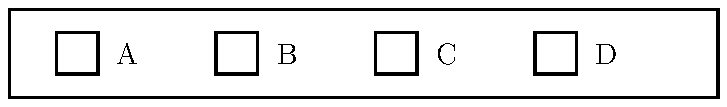
\includegraphics[width=0.85\textwidth]{choice4box}%
  \par\vspace{0.45cm}%
}

\begin{document}
\fiducials

\vspace*{0.5cm}

\begin{center}
  {\Large\textbf{Elementary Math Quiz}}\\[0.15cm]
  {\normalsize Name:\enspace\underline{\hspace{5.5cm}}\qquad Date:\enspace\underline{\hspace{2.8cm}}}
\end{center}

\vspace{0.2cm}

\noindent\textbf{Instructions:} Fill \textbf{exactly one} checkbox per question using a dark pen or pencil.
Fill the box completely. If you change your answer, erase the old mark cleanly before filling a new box.

\vspace{0.2cm}
\hrule
\vspace{0.35cm}

\mcq{1}{What is $7 + 5$?}{10}{11}{12}{13}

\mcq{2}{What is $15 - 8$?}{6}{7}{8}{9}

\mcq{3}{What is $4 \times 6$?}{20}{22}{24}{26}

\mcq{4}{What is $36 \div 4$?}{7}{8}{9}{10}

\mcq{5}{Which of these numbers is even?}{13}{17}{21}{24}

\end{document}
